\section{
A local equivalence
}
\draftnote{blue}{Consider}{
Put into own chapter?
Beyond SBDRL II: local algebras
}
\draftnote{green}{Include}{
\begin{enumerate}
    \item General properties of $(\hat{A}^{*}, \circ_{\sim_{w}})$.
\end{enumerate}
}

\begin{definition}[Local equivalence of actions under $\sim_{w}$]
	Given two actions $a, a' \in \hat{A}^{*}$ and a world state $w \in W$,
	\begin{equation}
		a \sim_{w} a' \iff a \ast w = a' \ast w
	\end{equation}
\end{definition}

\begin{proposition}
    $\sim_{w}$ is an equivalence relation.
\end{proposition}
\begin{proof}
    To prove that $\sim_{w}$ is an equivalence relation on the set $\hat{A}^{*}$, we need to show that $\sim_{w}$ is (1) reflexive, (2) symmetric, and (3) transitive.
    \begin{enumerate}[(1)]
        \item \textbf{Reflexive.}
        We need to show that $a \sim_{w} a$ for all $a \in \hat{A}^{*}$.
        By the definition of $\sim_{w}$, we need to check if $a \ast w = a \ast w$, which is true by equality.

        \item \textbf{Symmetric.}
        We need to show that if $a \sim_{w} a'$, then $a' \sim_{w} a$.
        If $a \sim_{w} a'$ then, by the definition of $\sim_{w}$, we have $a \sim_{w} a' \iff a \ast w = a' \ast w$.
        Therefore, we have that $a' \ast w = a \ast w$, and so, from the definition of $\sim_{w}$, we have $a' \sim_{w} a$.

        \item \textbf{Transitive.}
        We need to show that if $a \sim_{w} a'$ and $a' \sim_{w} a''$, then $a \sim_{w} a''$.
        Let $a \sim_{w} a'$ and $a' \sim_{w} a''$.
        By definition of $\sim_{w}$ we have $a \ast w = a' \ast w$ and $a' \ast w = a'' \ast w$.
        By transitivity of equality, we have $a \ast w = a'' \ast w$, which means $a \sim_{w} a''$.
    \end{enumerate}
\end{proof}

\begin{proposition}\label{prp:global_equivalence_implies_local_equivalence}
    For all $a, a' \in \hat{A}^{*}$,
    \begin{equation}
        a \sim a' \implies a \sim_{w} a' \quad \text{for all $w \in W$}
    \end{equation}
\end{proposition}
\begin{proof}
    If $a \sim a'$, then
    \begin{equation}
        \label{eqn:local_global_equivalence_1}
        a \ast w = a' \ast w \quad \text{for all $w \in W$}
    \end{equation}
    Select an arbitrary $w_{0} \in W$.
    From \cref{eqn:local_global_equivalence_1}, we have
    \begin{equation}
        a \ast w_{0} = a' \ast w_{0}
    \end{equation}
    By definition of local equivalence, we have
    \begin{equation}
        a \sim_{w_{0}} a'
    \end{equation}
    Since $w_{0}$ was an arbitrary choice, this argument holds for all $w \in W$, and so we have
    \begin{equation}
        a \sim_{w} a' \quad \text{for all $w \in W$}
    \end{equation}
\end{proof}


\begin{proposition}
    \begin{equation}
        a \sim a' \iff a \sim_{w} a' \quad \text{for all $w \in W$}
    \end{equation}
    \footnote{
    This means that $\sim$ is the intersection of all local equivalence relations
    \begin{equation}
        \sim \; = \bigcap_{w \in W} \sim_{w}
    \end{equation}
    \draftnote{blue}{Consider}{Can we draw this for our example ?}
    }
\end{proposition}
\begin{proof}
\begin{enumerate}[(1)]
    \item \textbf{$a \sim a' \implies a \sim_{w} a'$ for all $w \in W$.}
    See \cref{prp:global_equivalence_implies_local_equivalence}.

    \item \textbf{$a \sim a' \impliedby a \sim_{w} a'$ for all $w \in W$.}
    If $a \sim_{w} a'$ for all $w \in W$, then
    \begin{equation}
        \label{eqn:local_global_equivalence_2}
        a \ast w = a' \ast w \quad \text{for all $w \in W$}
    \end{equation}
    \cref{eqn:local_global_equivalence_2} is the definition of $a \sim a'$.
\end{enumerate}
\end{proof}

\draftnote{blue}{Move this}{
For a world state $w$ of a world $\mathscr{W}$, let $(\hat{A}^{*}/\sim)_{w}$ denote the set $\hat{A}^{*}/\sim$ of equivalence classes of $\hat{A}^{*}$ under the global equivalence $\sim$ for the reachable subworld $\mathscr{W}^{\hat{A}\to}(w)$ from $w$.
}

\begin{proposition}\label{prp:local_class_is_disjoint_union_of_global_classes}
    Every local equivalence class $[a]_{\sim_{w}} \in \hat{A}^{*}/\sim_{w}$ is a disjoint union of global equivalence classes\footnote{
    In other words, each local equivalence class in $\hat{A}^{*}/\sim_{w}$ is made up of one or more global equivalence classes in $\hat{A}^{*}/\sim$ and each global equivalence class in is exactly one local equivalence class.
    }
    \begin{equation}
        [a]_{\sim_{w}} = \bigsqcup_{i \in I}[a_{i}]_{\sim}
    \end{equation}
    where $\{ [a_{i}]_{\sim} \}_{i \in I} \subseteq \hat{A}^{*}/\sim$ and $[a_{i}]_{\sim} \subseteq [a]_{\sim_{w}}$ for all $i \in I$.
    \footnote{
    $I$ is the index set that labels all global equivalence classes contained in $[a]_{\sim_{w}}$:
    \begin{equation}
        I := \{ i \mid [a_{i}]_{\sim} \subseteq [a]_{\sim_{w}} \}
    \end{equation}
    }
\end{proposition}
\begin{proof}
\begin{enumerate}[(1)]
    \item \textbf{Global equivalence $\implies$ local equivalence.}
    From \cref{prp:global_equivalence_implies_local_equivalence} we have
    \begin{align}
        & a \sim a' \implies a \sim_{w} a' \\
        \implies & [a]_{\sim} \subseteq [a]_{\sim_{w}}
    \end{align}
    Therefore, each global equivalence class $[a_{i}]_{\sim}$ is contained entirely within a single local equivalence class $[a]_{\sim_{w}}$.
    Since each $[a_{i}]_{\sim} \subseteq [a]_{\sim_{w}}$, the union of all the $[a_{i}]_{\sim}$ contained in a specific $[a]_{\sim_{w}}$ is also contained in $[a]_{\sim_{w}}$.
    Therefore, we have
    \begin{equation}\label{eqn:subset1}
        \bigcup_{i \in I}[a_{i}]_{\sim} \subseteq [a]_{\sim_{w}}
    \end{equation}

    \item \textbf{Equality of sets.}
    For any $a' \in [a]_{\sim_{w}}$, we have $a' \sim_{w} a$ by definition.
    Since $a' \sim_{w} a$, we have $[a']_{\sim} \subseteq [a]_{\sim_{w}}$ (from step 1 of this proof).
    The index set $I$ labels all the global equivalence classes contained in $[a]_{\sim_{w}}$:
    \begin{equation}
        I = \{ i \mid [a_{i}]_{\sim} \subseteq [a]_{\sim_{w}} \}
    \end{equation}
    $I$ is well-defined because each global class is contained in exactly one local class.
    Since $[a']_{\sim} \subseteq [a]_{\sim_{w}}$, $[a']_{\sim}$ is one of the classes $[a_{i}]_{\sim}$ indexed by $I$.
    Therefore, $[a']_{\sim} \subseteq \bigcup_{i \in I}[a_{i}]_{\sim}$.
    Since $a' \in [a']_{\sim}$, we have $a' \in \bigcup_{i \in I}[a_{i}]_{\sim}$.
    Since $a'$ was an arbitrary element in $[a]_{\sim_{w}}$, we have
    \begin{equation}\label{eqn:subset2}
        [a]_{\sim_{w}} \subseteq \bigcup_{i \in I}[a_{i}]_{\sim}
    \end{equation}
    Combining \cref{eqn:subset1,eqn:subset2} gives
    \begin{equation}
        [a]_{\sim_{w}} = \bigcup_{i \in I}[a_{i}]_{\sim}
    \end{equation}
    
    \item \textbf{Disjointness of global equivalence classes.}
    \begin{enumerate}
        \item \textbf{Claim.}
        If $[a_{i}]_{\sim}$ and $[a_{j}]_{\sim}$ are distinct global equivalence classes contained within the same local equivalence class $[a]_{\sim_{w}}$, then they are disjoint
        \begin{equation}
            [a_{i}]_{\sim} \cap [a_{j}]_{\sim} = \emptyset
        \end{equation}

        \item \textbf{Proof by contradiction.}
        Assume that $[a_{i}]_{\sim}$ and $[a_{j}]_{\sim}$ are distinct global equivalence classes with a common element $b \in \hat{A}^{*}$ such that $b \in [a_{i}]_{\sim} \cap [a_{j}]_{\sim}$.
        By definition of equivalence classes, we have
        \begin{align}
            & b \in [a_{i}]_{\sim} \implies b \sim a_{i} \\
            & b \in [a_{j}]_{\sim} \implies b \sim a_{j}
        \end{align}
        By transitivity of $\sim$, we have
        \begin{align}
            & a_{i} \sim b \sim a_{j} \\
            \implies & a_{i} \sim a_{j} \\
            \implies & [a_{i}]_{\sim} = [a_{j}]_{\sim}
        \end{align}
        This contradicts that $[a_{i}]_{\sim}$ and $[a_{j}]_{\sim}$ are distinct.
    \end{enumerate}

    \item \textbf{Conclusion.}
    The union $\bigcup_{i \in I}[a_{i}]_{\sim}$ is (1) equal to $[a]_{\sim_{w}}$, and (2) disjoint.
    Therefore, we have
    \begin{equation}
        [a]_{\sim_{w}} = \bigsqcup_{i \in I}[a_{i}]_{\sim}
    \end{equation}
\end{enumerate}
\end{proof}



\draftnote{blue}{Footnote}{
The global equivalence $\sim$ is a refinement of the local equivalences $\sim_{w}$ for $w \in W$; this means that globally equivalent actions must be locally equivalence, but locally equivalent action do not need to be globally equivalent.
\begin{align}
    a \sim a' & \implies a \sim_{w} a' \\
    a \sim_{w} a' & \nRightarrow a \sim a'
\end{align}
}



We attempt to define our induced composition operator $\circ_{\sim_{w}}$ on the quotient set $\hat{A}^{*}/\sim_{w}$ in a similar way to how we defined the composition operator $\circ_{\sim}$ for our global equivalence relation $\sim$:
\begin{equation}
\begin{aligned}
    \circ_{\sim_{w}}: \; &(\hat{A}^{*}/\sim_{w}) \times (\hat{A}^{*}/\sim_{w}) \to (\hat{A}^{*}/\sim_{w}) \quad \text{such that}\\
    & [a']_{\sim_{w}} \circ_{\sim_{w}} [a]_{\sim_{w}} := [a' \circ a]_{\sim_{w}}
\end{aligned}
\end{equation}


%%%%%%%%%%%%%%%%%%%%%%%%%%%%%%%%%%%%%%%%%%%%%
\section{Local algebra algorithm}
\draftnote{green}{Include}{
\begin{enumerate}
        \item (?) Put the full algorithm in the appendices.
        \item CODE: well-definedness checker ?
\end{enumerate}
}

As with $\sim$, we developed an algorithm to construct the quotient set $\hat{A}^{*}/\sim_{w}$ and construct a Cayley table of the algebra $(\hat{A}^{*}/\sim_{w}, \circ_{\sim_{w}})$.

The latest version of the code for this section can be found at
\begin{center}
\url{https://github.com/awjdean/CayleyTableGeneration}
\end{center}

%%%%%%%%%%%%%%%%%%%%%%%%%%%%%%%%%%%%%%%%%%%%%
\subsection{Generating the equivalence classes}

To generate the local algebra, we altered algorithm \ref{alg:GenerateEquivClasses} to use a different $\Call{ComputeActionFunction}$ function.
Since our $\Call{LocalComputeActionFunction}$ requires an additional initial state parameter $w^{*}$, we must also feed that parameter into $\Call{GenerateEquivClasses}$ and $\Call{ProcessCandidate}$.
Other than those changes, the algorithm for generating the equivalence classes for the local algebra is the same as for the global algebra.

\begin{algorithm}[H]
	\caption{
		Compute the part of the action function $f_{a}: W \to W$ that sends $w^{*} \mapsto a \ast w^{*}$.
	}
    \label{alg:LocalComputeActionFunction}
	\hrulefill
	\begin{algorithmic}[1]
		\Procedure{LocalComputeActionFunction}{$a$, \; $\mathscr{W}$, \; $w^{*}$}
		\State $f_{a} \gets (\emptyset \to \emptyset)$
		\State $w_{a} \gets$ \Call{GenerateActionOutcome}{$a$, \; $w^{*}$, \; $\hat{\ast}$}
		\State $f_{a} \gets f_{a} \cup f_{a}'$ where $f_{a}': \{w^{*}\} \to \{w_{a}\}$ such that $f_{a}'(w^{*}) = w_{a}$
		\State \Return $f_{a}$
		\EndProcedure
	\end{algorithmic}
\end{algorithm}

%%%%%%%%%%%%%%%%%%%%%%%%%%%%%%%%%%%%%%%%%%%%%
\subsection{Generating the Cayley table}

To generate the local Cayley table, we use algorithm \ref{alg:GenerateCayley} with a different $\Call{ComputeCompositionActionFunction}$ function.

\begin{algorithm}[H]
	\caption{
		Compute the action function for the combination $l_{L} \circ l_{R}$ using \Call{LocalComputeActionFunction}.
	}
        \label{alg:ComputeCompositionActionFunction_local}
	\hrulefill
	\begin{algorithmic}[1]
		\Procedure{ComputeCompositionActionFunction}{$l_{L}$, \; $l_{R}$, \; $\mathcal{T}$, \; $\rho$, \; $\mathscr{W}$, \; $w^{*}$}
		      \State $a \gets \operatorname{Combine}(l_{L}, \; l_{R})$
                \State $f_{a} \gets$ \Call{LocalComputeActionFunction}{$a$, \; $\mathscr{W}$, \; $w^{*}$}
                \State \Return $f_{a}$
		\EndProcedure
	\end{algorithmic}
\end{algorithm}


%%%%%%%%%%%%%%%%%%%%%%%%%%%%%%%%%%%%%%%
\subsection{Mathematical analysis}

\begin{proposition}\label{prp:local_algebra_cardinality}
The number of elements in $\hat{A}^{*}/\sim_{w}$ is the number of world states that are reachable from $w$.
    \begin{equation}
        |\hat{A}^{*}/\sim_{w}| = |W^{\hat{A}\to}(w)| \leq |W|
    \end{equation}
\end{proposition}
\begin{proof}
\begin{enumerate}[(1)]
    \item \textbf{Define mapping between $\hat{A}^{*}/\sim_{w}$ and $W^{\hat{A}\to}(w)$.}
    We define the canonical mapping
    \begin{equation}
    \begin{aligned}
        & \phi: \hat{A}^{*}/\sim_{w} \to W^{\hat{A}\to}(w) \\
        & \phi([a]_{\sim_{w}}) = a \ast w
    \end{aligned}
    \end{equation}

    \item \textbf{Injectivity of $\phi$.}
    \begin{align}
        & \phi([a]_{\sim_{w}}) = \phi([a']_{\sim_{w}}) \\
        \implies & a \ast w = a' \ast w \\
        \implies & a \sim_{w} a' \\
        \implies & [a]_{\sim_{w}} = [a']_{\sim_{w}}
    \end{align}
    Therefore $\phi$ is injective.

    \item \textbf{Subjectivity of $\phi$.}
    Consider an arbitrary world state $w' \in W^{\hat{A}\to}(w)$.
    By the definition of $W^{\hat{A}\to}(w)$, there exists at least one action sequence $a \in \hat{A}^{*}$ such that $a \ast w = w'$.
    Therefore, $\phi([a]_{\sim_{w}}) = a \ast w = w'$.
    Since the choice of $w' \in W^{\hat{A}\to}(w)$ is arbitrary, there exists an equivalence class $[a]_{\sim_{w}} \in \hat{A}^{*}/\sim_{w}$ such that $\phi([a]_{\sim_{w}}) = w'$ for all world states in $W^{\hat{A}\to}(w)$.
    Therefore, $\phi$ is surjective.

    \item \textbf{Bijectivity of $\phi$}
    Since $\phi$ is injective and surjective, $\phi$ is bijective and therefore
    \begin{equation}
        |\hat{A}^{*}/\sim_{w}| = |W^{\hat{A}\to}(w)|
    \end{equation}
    $|W^{\hat{A}\to}(w)| \leq |W| + 1$ from the definition of $W^{\hat{A}\to}(w)$.
\end{enumerate}
\end{proof}

\begin{proposition}
    \Cref{alg:GenerateEquivClasses} with adjustments for the local equivalence $\sim_{w}$ (\cref{alg:LocalComputeActionFunction,alg:ComputeCompositionActionFunction_local}) always halts for finite $W$.
\end{proposition}
\begin{proof}
\begin{enumerate}[(1)]
    \item \textbf{$|L|$ increases monotonically until its final iteration.}
    During each expansion iteration, the set $L$ either grows or remains the same.
    So at each expansion iteration, with a new distinct action is discovered and added to $L$ or no new distinct actions are discovered and the algorithm halts.

    \item \textbf{Upper bound on $|L|$.}
    Each equivalence class $[a]_{\sim_{w}} \in L$ is uniquely determined by its effect on $w^{*}$.
    For a world with $|W|$ world states there are at most $|W| + 1$ distinct transformations with a source of $w^{*}$ (one to every world state in $W^{\bot}$)\footnote{
    As we know from \cref{prp:local_algebra_cardinality} there are actually at most $|W^{\hat{A}\to}(w^{*})|$ distinct transformations with a source of $w^{*}$.
    }.
    Therefore, the set $L$ can have at most $|W|+1$ elements.

    \item \textbf{Halting.}
    If $L$ stops growing for one expansion iteration, then the algorithm halts.
    If $|L| = |W|+1$, then there are no more unique action functions and therefore no more distinct actions under $\sim_{w}$ and so \cref{alg:GenerateEquivClasses} halts.
    Since $|L|$ increases monotonically when it changes, either $|L|$ reaches $|W|+1$ and halts or the algorithm halts before $|L|=|W|+1$.
\end{enumerate}
\end{proof}

\begin{proposition}
    Consider \cref{alg:GenerateEquivClasses} with adjustments for the local equivalence $\sim_{w}$ (\cref{alg:LocalComputeActionFunction,alg:ComputeCompositionActionFunction_local}).
    When this algorithm halts, $L \cong \hat{A}^{*}/\sim_{w}$
\end{proposition}
\begin{proof}
    \textbf{Proof by contradiction.}
\begin{enumerate}[(1)]
    \item \textbf{Set up.}
    Assume the algorithm halts with a set $L$, but there exists an undiscovered equivalence class $[b]_{\sim_{w}} \in \hat{A}^{*}/\sim_{w}$.
    Let $b$ be the shortest action such that $b \ast w^{*}$ is not represented in $L$ (i.e., $b$ is the shortest distinct action under $\sim_{w}$).

    \item \textbf{Decomposition of $b$.}
    We can write $b$ as $b = \hat{a} \circ b'$ where $\hat{a} \in \hat{A}/\sim_{w}$ and $b' \in \hat{A}^{\ast}$.
    Since $b$ is the shortest undiscovered distinct action under $\sim_{w}$, either $b'$ must have been discovered and be represented in $L$ or $b'$ is not discovered and $b$ is not the shortest undiscovered distinct action under $\sim_{w}$, since $b'$ is shorter than $b$, which is a contradiction.

    \item \textbf{Contradiction.}
    Given that $b'$ is known and represented in $L$, the algorithm will have left composed $b'$ with every distinct minimum action in $\hat{A}/\sim_{w}$, including $\hat{a}$.
    Therefore, the algorithm must have discovered $b = \hat{a} \circ b'$, which is a contradiction.
\end{enumerate}
\end{proof}

\paragraph{Complexity analysis.}
Let $|W|=n$ and let $|\hat{A}/\sim_{w}|=m$.
In the worst case, all world states are reachable ($|W^{\hat{A}\to}(w)| = |W|$) and so \cref{alg:GenerateEquivClasses} with adjustments for the local equivalence $\sim_{w}$ (\cref{alg:LocalComputeActionFunction,alg:ComputeCompositionActionFunction_local}) must apply all $m$ distinct minimum actions under $\hat{A}/\sim_{w}$ to each world state.
Therefore, the upper bound on the time complexity of \cref{alg:GenerateEquivClasses} with adjustments for the local equivalence $\sim_{w}$ (\cref{alg:LocalComputeActionFunction,alg:ComputeCompositionActionFunction_local}) is
\begin{equation}
    \mathcal{O}(m \cdot n)
\end{equation}


%%%%%%%%%%%%%%%%%%%%%%%%%%%%%%%%%%%%%%%
\section{
Action homogeneity
}
%%%%%%%%%%%%%%%%%%%%%%%%%%%%%%%%%%%%%%%
\subsection{
A motivating example
}
\draftnote{green}{To do}{
\begin{enumerate}
    \item Talk about differences between $\mathscr{W}_{\alpha}$ vs $\mathscr{W}_{\beta}$ with identity treatment.
\end{enumerate}
}

\begin{table}[H]
    \centering
    \begin{tabular}{cc}
        \subcaptionbox{$w_{0}$\label{tab:W_alpha_local_w0_cayley}}{
            \begin{tabularx}{0.6\textwidth}{l|llll}
$\circ_{\sim_{w_{0}}}$ & $[1]$ & $[W]$ & $[N]$ & $[NW]$ \\
\hline
$[1]$ & $[1]$ & $[W]$ & $[N]$ & $[NW]$ \\
$[W]$ & $[W]$ & $[1]$ & $[NW]$ & $[N]$ \\
$[N]$ & $[N]$ & $[NW]$ & $[1]$ & $[W]$ \\
$[NW]$ & $[NW]$ & $[N]$ & $[W]$ & $[1]$ \\
\end{tabularx}

        } &
        \subcaptionbox{$w_{1}$}{
            \begin{tabularx}{0.6\textwidth}{l|llll}
$\circ_{\sim_{w_{1}}}$ & $[1]$ & $[W]$ & $[N]$ & $[NW]$ \\
\hline
$[1]$ & $[1]$ & $[W]$ & $[N]$ & $[NW]$ \\
$[W]$ & $[W]$ & $[1]$ & $[NW]$ & $[N]$ \\
$[N]$ & $[N]$ & $[NW]$ & $[1]$ & $[W]$ \\
$[NW]$ & $[NW]$ & $[N]$ & $[W]$ & $[1]$ \\
\end{tabularx}

        } \\
        \subcaptionbox{$w_{2}$}{
            \begin{tabularx}{0.6\textwidth}{l|llll}
$\circ_{\sim_{w_{2}}}$ & $[1]$ & $[W]$ & $[N]$ & $[NW]$ \\
\hline
$[1]$ & $[1]$ & $[W]$ & $[N]$ & $[NW]$ \\
$[W]$ & $[W]$ & $[1]$ & $[NW]$ & $[N]$ \\
$[N]$ & $[N]$ & $[NW]$ & $[1]$ & $[W]$ \\
$[NW]$ & $[NW]$ & $[N]$ & $[W]$ & $[1]$ \\
\end{tabularx}

        } &
        \subcaptionbox{$w_{3}$}{
            \begin{tabularx}{0.6\textwidth}{l|llll}
$\circ_{\sim_{w_{3}}}$ & $[1]$ & $[W]$ & $[N]$ & $[NW]$ \\
\hline
$[1]$ & $[1]$ & $[W]$ & $[N]$ & $[NW]$ \\
$[W]$ & $[W]$ & $[1]$ & $[NW]$ & $[N]$ \\
$[N]$ & $[N]$ & $[NW]$ & $[1]$ & $[W]$ \\
$[NW]$ & $[NW]$ & $[N]$ & $[W]$ & $[1]$ \\
\end{tabularx}

        }
    \end{tabular}
    \caption{
    Constructions of local Cayley tables of $(\hat{A}^{*}/\sim_{w_{i}}, \circ_{\sim_{w_{i}}})$ for an agent with $\hat{A} = \{1, E, W, N, S \}$ in world $\mathscr{W}_{\alpha}$.
    \draftnote{blue}{To do}{Sort table formatting.}
    }
    \label{tab:W_alpha_local_cayley_tables}
\end{table}

As we can see from \cref{tab:W_alpha_local_cayley_tables}, all the constructions\footnote{
There's a reason we say "constructions" here; this will become clear later.
} of local Cayley tables are the same for the world $\mathscr{W}_{\alpha}$ and each of them forms the same Abelian group (see \cref{tab:W_alpha_local_algebra_properties}).
In fact, the local algebra $(\hat{A}^{*}/\sim_{w_{i}}, \circ_{\sim_{w_{i}}})$ is isomorphic to the global algebra $(\hat{A}^{*}/\sim, \circ_{\sim})$.
\draftnote{blue}{To do}{
Table comparing local algebra with global algebra for $\mathscr{W}_{\alpha}$.
}

\begin{table}[H]
\centering
\begin{tabular}{lc}
    \hline
    \textbf{Property} & \textbf{Present?} \\
    \hline
    Total & Y \\
    Associative & Y \\
    Identity & Y \\
    Inverses & Y \\
    \hline
    Commutative & Y \\
\end{tabular}
\caption{
Properties of $(\hat{A}^{*}/\sim_{w_{i}}, \circ_{\sim_{w_{i}}})$, where $i = 0, 1, 2, 3$, for an agent with $\hat{A} = \{1, E, W, N, S \}$ in world $\mathscr{W}_{\alpha}$.
\draftnote{blue}{To do}{Sort table formatting.}
}
\label{tab:W_alpha_local_algebra_properties}
\end{table}

But what about world $\mathscr{W}_{\beta}$ with identity treatment ?

\begin{table}[H]
    \centering
    \begin{tabular}{cc}
        \subcaptionbox{$w_{0}$\label{tab:W_beta_identity_local_w0_cayley}}{
            \begin{tabularx}{0.6\textwidth}{l|llll}
$\circ_{\sim_{w_{0}}}$ & $[1]$ & $[W]$ & $[N]$ & $[NW]$ \\
\hline
$[1]$ & $[1]$ & $[W]$ & $[N]$ & $[NW]$ \\
$[W]$ & $[W]$ & $[W]$ & $[NW]$ & $[N]$ \\
$[N]$ & $[N]$ & $[NW]$ & $[1]$ & $[W]$ \\
$[NW]$ & $[NW]$ & $[NW]$ & $[W]$ & $[1]$ \\
\end{tabularx}

        } &
        \subcaptionbox{$w_{1}$}{
            \begin{tabularx}{0.6\textwidth}{l|llll}
$\circ_{\sim_{w_{1}}}$ & $[1]$ & $[E]$ & $[N]$ & $[NE]$ \\
\hline
$[1]$ & $[1]$ & $[E]$ & $[N]$ & $[NE]$ \\
$[E]$ & $[E]$ & $[E]$ & $[NE]$ & $[N]$ \\
$[N]$ & $[N]$ & $[NE]$ & $[1]$ & $[E]$ \\
$[NE]$ & $[NE]$ & $[NE]$ & $[E]$ & $[1]$ \\
\end{tabularx}

        } \\
        \subcaptionbox{$w_{2}$}{
            \begin{tabularx}{0.6\textwidth}{l|llll}
$\circ_{\sim_{w_{2}}}$ & $[1]$ & $[W]$ & $[N]$ & $[NW]$ \\
\hline
$[1]$ & $[1]$ & $[W]$ & $[N]$ & $[NW]$ \\
$[W]$ & $[W]$ & $[1]$ & $[NW]$ & $[NW]$ \\
$[N]$ & $[N]$ & $[NW]$ & $[1]$ & $[W]$ \\
$[NW]$ & $[NW]$ & $[N]$ & $[W]$ & $[W]$ \\
\end{tabularx}

        } &
        \subcaptionbox{$w_{3}$}{
            \begin{tabularx}{0.6\textwidth}{l|llll}
$\circ_{\sim_{w_{3}}}$ & $[1]$ & $[W]$ & $[N]$ & $[NW]$ \\
\hline
$[1]$ & $[1]$ & $[W]$ & $[N]$ & $[NW]$ \\
$[W]$ & $[W]$ & $[1]$ & $[N]$ & $[NW]$ \\
$[N]$ & $[N]$ & $[NW]$ & $[1]$ & $[W]$ \\
$[NW]$ & $[NW]$ & $[N]$ & $[1]$ & $[1]$ \\
\end{tabularx}

        }
    \end{tabular}
    \caption{
    Constructions of local Cayley tables of $(\hat{A}^{*}/\sim_{w_{i}}, \circ_{\sim_{w_{i}}})$ for an agent with $\hat{A} = \{1, E, W, N, S \}$ in world $\mathscr{W}_{\beta}$ with identity treatment.
    \draftnote{blue}{To do}{Sort table formatting.}
    }
    \label{tab:W_beta_identity_local_cayley_tables}
\end{table}

The constructions of the local Cayley tables for $\mathscr{W}_{\beta}$ with the identity treatment are all different (see \cref{tab:W_beta_identity_local_cayley_tables}).

\begin{table}[H]
\centering
\begin{tabular}{lcccc}
    \hline
    \multirow{2}{*}{\textbf{Property}} & \multicolumn{4}{c}{\textbf{Present?}} \\
            & $w_{0}$   & $w_{1}$   & $w_{2}$   & $w_{3}$ \\
    \hline
    Total   & Y         & Y         & Y         & Y \\
    Associative & N     & N         & N         & N \\
    Identity & Y        & Y         & Y         & Y \\
    Inverses & N        & N         & N         & Y \\
    \hline
    Commutative & N     & N         & N         & N \\
\end{tabular}
\caption{
Properties of constructions of Cayley tables for $(\hat{A}^{*}/\sim_{w_{i}}, \circ_{\sim_{w_{i}}})$, where $i = 0, 1, 2, 3$, for an agent with $\hat{A} = \{1, E, W, N, S \}$ in world $\mathscr{W}_{\beta}$ with identity.
\draftnote{blue}{To do}{Sort table formatting.}
}
\label{tab:W_beta_identity_local_algebra_properties}
\end{table}
\draftnote{blue}{To do}{
Associativity is difficult to pick out from the observation of a Cayley table, so table ??? shows examples of associativity breaking for each $(\hat{A}^{*}/\sim_{w_{i}}, \circ_{\sim_{w_{i}}})$....
}


\draftnote{blue}{To do}{
Include $\mathscr{W}_{\beta}$ with masked treatment ?
}


%%%%%%%%%%%%%%%%%%%%%%%%%%%%%%%%%%%%%%%
\subsection{What's happening with the local equivalence $\sim_{w}$?}

The reason for the differences in the constructions of the Cayley tables for the world $\mathscr{W}_{\beta}$ with identity treatment is that the operation $\circ_{\sim_{w}}$ is not always well-defined on $\hat{A}^{*}/\sim_{w}$.

\begin{proposition}
    $\circ_{\sim_{w}}$ is \textbf{not} generally well-defined on $\hat{A}^{*}/\sim_{w}$.
\end{proposition}
\begin{proof}
\begin{enumerate}[(1)]
    \item \textbf{Problem.}
    For $\circ_{\sim_{w}}$ to be well-defined on $\hat{A}^{*}/\sim_{w}$, we need that
    \begin{equation}
    \begin{aligned}
        & \text{If $a \sim_{w} b$ and $a' \sim_{w} b'$, then} \\
        & (a' \circ a) \sim_{w} (b' \circ b) \quad \text{for all $a, b, a', b' \in \hat{A}^{*}$}
    \end{aligned}
    \end{equation}

    \item \textbf{Counter example: set up.}
    \draftnote{blue}{To do}{Put minimum action diagram of relevant transformations in margin.}
    Consider a world-agent pair $\mathscr{W}$-$\mathscr{A}$ with $W = \{w, w_{1}, w_{2}, w_{3}, w_{4} \}$, $\hat{A} = \{ \hat{a}_{1}, \hat{a}_{2}, \hat{a}'_{1}, \hat{a}'_{2} \}$, and $\hat{\circ}$ given by
    \begin{table}[H]
        \centering
        \begin{tabular}{c|ccccc}
           $\hat{\circ}$    & $w$       & $w_{1}$   & $w_{2}$   & $w_{3}$   & $w_{4}$ \\
           \hline
           $\hat{a}_{1}$    & $w_{1}$   & -         & -         & -         & - \\
           $\hat{a}_{2}$    & $w_{1}$   & -         & -         & -         & - \\
           $\hat{a}'_{1}$   & $w_{2}$   & $w_{3}$   & -         & -         & - \\
           $\hat{a}'_{2}$   & $w_{2}$   & $w_{4}$   & -         & -         & - \\
        \end{tabular}
        \caption{
        \draftnote{blue}{To do}{Improve caption.}
        Table entries with "-" are not relevant to the proof and can send the relevant world state to any world state in $W$.
        }
    \end{table}

    \item \textbf{Counter example: proof.}
    \begin{align}
        & \hat{a}_{1} \ast w = w_{1} \; \text{and} \; \hat{a}_{2} \ast w = w_{1} \implies \hat{a}_{1} \sim_{w} \hat{a}_{2} \\
        & \hat{a}'_{1} \ast w = w_{1} \; \text{and} \; \hat{a}'_{2} \ast w = w_{1} \implies \hat{a}'_{1} \sim_{w} \hat{a}'_{2}
    \end{align}
    But
    \begin{align}
        & (\hat{a}'_{1} \circ \hat{a}_{1}) \ast w = \hat{a}'_{1} \ast (\hat{a}_{1} \ast w) = \hat{a}'_{1} \ast w_{1} = w_{3} \\
        & (\hat{a}'_{2} \circ \hat{a}_{2}) \ast w = \hat{a}'_{2} \ast (\hat{a}_{2} \ast w) = \hat{a}'_{2} \ast w_{1} = w_{4}
    \end{align}
    which gives
    \begin{equation}
        (\hat{a}'_{1} \circ \hat{a}_{1}) \not\sim_{w} (\hat{a}'_{2} \circ \hat{a}_{2})
    \end{equation}
\end{enumerate}
\end{proof}

Since $\circ_{\sim_{w}}$ is not generally well-defined on $\hat{A}^{*}/\sim_{w}$, we cannot generally construct an algebra $(\hat{A}^{*}/\sim_{w}, \circ_{\sim_{w}})$ because the elements in each equivalence class in $\hat{A}^{*}/\sim_{w}$ do not always behave in the same way as each other under $\circ$ if we apply $\sim_{w}$ to the result \draftnote{blue}{Consider}{Reword the end of this ?}.
In other words,
\begin{equation}
    \text{In general,} \quad [a']_{\sim_{w}} \circ_{\sim_{w}} [a]_{\sim_{w}} \neq [a' \circ a]_{\sim_{w}}
\end{equation}

The reason that $\circ_{\sim_{w}}$ is not generally well-defined is that the local equivalence $\sim_{w}$ captures the effect of actions on the world state $w$; $\sim_{w}$ does not capture the effect of actions on other states, which might act as intermediaries when considering the result of composing actions under $\sim_{w}$.


\draftnote{blue}{To do}{
Something about the definition of $\circ_{\sim_{w}}$ being $a' \circ_{\sim_{w}} a = [a' \circ a]_{\sim_{w}}$ in the not well-defined case.
}



%%%%%%%%%%%%%%%%%%%%%%%%%%%%%%%%%%%%%%%
\subsection{Some proofs}

\begin{proposition}\label{prp:circ_local_well_defined_implies_circ_local_associative}
    $\circ_{\sim_{w}}$ is well-defined on $\hat{A}^{*}/\sim_{w}$ $\implies$ $\circ_{\sim_{w}}$ is associative on $\hat{A}^{*}/\sim_{w}$.
    \draftnote{blue}{Include as footnote}{This is a property of universal algebra.}
\end{proposition}
\begin{proof}
\begin{enumerate}[(1)]
    \item \textbf{Set up.}
    If $\circ_{\sim_{w}}$ is well-defined on $\hat{A}^{*}/\sim_{w}$, we have
    \begin{equation}\label{eqn:circ_sim_well_defined_associative}
        [a']_{\sim_{w}} \circ_{\sim_{w}} [a]_{\sim_{w}} = [a' \circ a]_{\sim_{w}}
    \end{equation}

    We want to show that for any equivalence classes $[a]_{\sim_{w}}, [a']_{\sim_{w}}, [a'']_{\sim_{w}} \in \hat{A}^{*}/\sim_{w}$
    \begin{equation}
        ([a]_{\sim_{w}} \circ [a']_{\sim_{w}}) \circ [a'']_{\sim_{w}} = [a]_{\sim_{w}} \circ ([a']_{\sim_{w}} \circ [a'']_{\sim_{w}})
    \end{equation}

    \item \textbf{LHS.}
    Using the well-defined property (\cref{eqn:circ_sim_well_defined_associative}), we have
    \begin{equation}
        ([a]_{\sim_{w}} \circ [a']_{\sim_{w}}) \circ [a'']_{\sim_{w}} = [(a \circ a') \circ a'']_{\sim_{w}}
    \end{equation}

    \item \textbf{RHS.}
    Similarly for the RHS, we have
    \begin{equation}
        [a]_{\sim_{w}} \circ ([a']_{\sim_{w}} \circ [a'']_{\sim_{w}}) = [a \circ (a' \circ a'')]_{\sim_{w}}
    \end{equation}
    \item \textbf{Combining LHS and RHS.}
    Using the associative property of $\circ$ on $\hat{A}^{*}$, we have
    \begin{equation}
        [(a \circ a') \circ a'']_{\sim_{w}} = [a \circ (a' \circ a'')]_{\sim_{w}}
    \end{equation}
\end{enumerate}
\end{proof}

Consider a set $A$ with a composition operator $\cdot$ that combines elements in $A$ as $\cdot: A \times A \to A$, and an equivalence relation $\sim$ on $A$.
Let the Cayley table with rows and columns labelled by the elements of this set $A$ and with entries given by $a \cdot b$ where $a$ is the row label of the entry and $b$ is the column label of the entry be denoted by $T(A, \cdot)$.
We denote by $T_{\sim}(A, \cdot)$ the Cayley table with rows and columns labelled by the elements of the quotient set $A/\sim$ and with entries given by $[a]_{\sim} \cdot_{\sim} [b]_{\sim} = [a \cdot b]_{\sim}$ where $a \in A$ is a representative element of the row label $[a]_{\sim} \in A/\sim$ and $b \in A$ is a representative element of the column label $[b]_{\sim} \in A/\sim$.


\begin{proposition}
    $\circ_{\sim_{w}}$ is well-defined $\iff$ the Cayley table $T_{\sim_{w}}(\hat{A}^{*}, \circ)$ has a single consistent value in each table entry\footnote{
    This means that there is one unique construction of the Cayley table $T_{\sim_{w}}(\hat{A}^{*}, \circ)$.
    }.
\end{proposition}
\begin{proof}
\begin{enumerate}[(1)]
    \item \textbf{$\circ_{\sim_{w}}$ is well-defined $\implies$ the Cayley table $T_{\sim_{w}}(\hat{A}^{*}, \circ)$ has a single consistent value in each table entry.}
    If $\circ_{\sim_{w}}$ is well-defined, then the value of $[a]_{\sim_{w}} \circ_{\sim_{w}} [a']_{\sim_{w}}$ does not depend on the choice of representative $a, b \in \hat{A}^{*}$, and so the composition $[a]_{\sim_{w}} \circ_{\sim_{w}} [a']_{\sim_{w}}$ is \textbf{uniquely} determined by the equivalence classes themselves and not by their representatives.
    Therefore, every entry in the Cayley table is a unique equivalence class in $\hat{A}^{*}/\sim_{w}$ independent of the choice of representative.

    \item \textbf{$\circ_{\sim_{w}}$ is well-defined $\impliedby$ the Cayley table $T_{\sim_{w}}(\hat{A}^{*}, \circ)$ has a single consistent value in each table entry.}
    If $T_{\sim_{w}}(\hat{A}^{*}, \circ)$ has a single consistent value in each table entry, then each entry $[a]_{\sim_{w}} \circ_{\sim_{w}} [a']_{\sim_{w}}$, which is computed as $[a \circ a']_{\sim_{w}}$ is unique, and so does not depend on the representative element; this is exactly the condition for $\circ_{\sim_{w}}$ being well-defined on $\hat{A}^{*}/\sim_{w}$.
\end{enumerate}
\end{proof}

\begin{corollary}
    $\circ_{\sim_{w}}$ is not well-defined $\iff$ there are multiple unique Cayley table constructions of $(\hat{A}^{*}/\sim_{w}, \circ_{\sim_{w}})$.
\end{corollary}


\begin{proposition}
    Associativity property not present in a Cayley table $T_{\sim_{w}}(\hat{A}^{*}, \circ)$ $\implies$ $\circ_{\sim_{w}}$ is not well-defined on $\hat{A}^{*}/\sim_{w}$.
\end{proposition}
\begin{proof}
\begin{enumerate}[(1)]
    \draftnote{blue}{Consider}{Not super happy with this proof.}
    \item \textbf{Algebraic argument.}
    If $\circ_{\sim_{w}}$ is well-defined, then, for any $a, a', a'' \in \hat{A}^{*}$, we have
    \begin{align}
          & ([a]_{\sim_{w}} \circ_{\sim_{w}} [a']_{\sim_{w}}) \circ_{\sim_{w}} [a'']_{\sim_{w}} \\
        = & [(a \circ a') \circ a'']_{\sim_{w}} \quad \text{(definition of $\circ_{\sim_{w}}$}) \\
        = & [a \circ (a' \circ a'')]_{\sim_{w}} \quad \text{(associativity of $\circ$}) \\
        = & [a]_{\sim_{w}} \circ_{\sim_{w}} ([a']_{\sim_{w}} \circ_{\sim_{w}} [a'']_{\sim_{w}}) \quad \text{(definition of $\circ_{\sim_{w}}$})
    \end{align}

    If $T_{\sim_{w}}(\hat{A}^{*}, \circ)$ does not satisfy the associativity property, then there exists $a, a', a'' \in \hat{A}^{*}$ such that
    \begin{equation}
        ([a]_{\sim_{w}} \circ_{\sim_{w}} [a']_{\sim_{w}}) \circ_{\sim_{w}} [a'']_{\sim_{w}} \neq [a]_{\sim_{w}} \circ_{\sim_{w}} ([a']_{\sim_{w}} \circ_{\sim_{w}} [a'']_{\sim_{w}})
    \end{equation}
    Since the associativity of $\circ$ is given, there must be an issue with the definition of $\circ_{\sim_{w}}$ (\textit{i.e.}, it depends on the on the choice of representative in $\hat{A}^{*}/\sim_{w}$.
    
    \item \textbf{Logic argument.}
    From \cref{prp:circ_local_well_defined_implies_circ_local_associative}, we have
    \begin{equation}
        \circ_{\sim_{w}} \; \text{well-defined on $\hat{A}^{*}/\sim_{w}$} \implies \circ_{\sim_{w}} \; \text{associative on $\hat{A}^{*}/\sim_{w}$}.
    \end{equation}
    By contrapositive we have
    \begin{equation}
        \neg(\circ_{\sim_{w}} \; \text{associative on $\hat{A}^{*}/\sim_{w}$}) \implies \neg(\circ_{\sim_{w}} \; \text{well-defined on $\hat{A}^{*}/\sim_{w}$})
    \end{equation}
    In other words,
    \begin{equation}
        \circ_{\sim_{w}} \; \text{\textbf{not} associative on $\hat{A}^{*}/\sim_{w}$} \implies \circ_{\sim_{w}} \; \text{\textbf{not} well-defined on $\hat{A}^{*}/\sim_{w}$}
    \end{equation}
    If $\circ_{\sim_{w}}$ is not associative on $\hat{A}^{*}/\sim_{w}$ 
\end{enumerate}    
\end{proof}

\draftnote{blue}{Include}{
Therefore, if a construction of the Cayley table $T_{\sim_{w}}(\hat{A}^{*}, \circ)$ does not satisfy associativity then $\circ_{\sim_{w}}$ as presented in the construction of the Cayley table does not coincide with a well-defined $\circ_{\sim_{w}}$.
This means there is no single well-defined binary operation on the quotient set $\hat{A}^{*}/\sim_{w}$ consistent with the underlying composition operator $\circ$ on $\hat{A}$.
}

\draftnote{blue}{Use}{
\begin{itemize}
    \item If $\circ_{\sim_{w}}$ is not well-defined, then constructions of the Cayley table $T_{\sim_{w}}(\hat{A}^{*}, \circ)$ are "representative specific".
\end{itemize}
}

\draftnote{blue}{Note about Cayley tables}{
For a Cayley table $T_{\sim}(\hat{A}^{*}, \circ)$
\begin{enumerate}
    \item Rows are labelled by the distinct classes $[x]_{\sim} \in \hat{A}^{*}/\sim$.
    \item Columns are labelled by the same distinct classes $[x]_{\sim} \in \hat{A}^{*}/\sim$ (with the same representative elements for those classes used).
    \item The table entry in row $[x]_{\sim}$ and column $[y]_{\sim}$ is filled with
    \begin{equation}
        [x]_{\sim} \circ_{\sim} [y]_{\sim} := [x \circ y]_{\sim}
    \end{equation}
    where $x$ is some representative in $[x]_{\sim}$ and $y$ is some representative in $[y]_{\sim}$.
    If $\circ_{\sim}$ is not well-defined, then different choices of representative may produce different outcomes in the Cayley table; this means if $\circ_{\sim}$ is not well-defined we can construct multiple Cayley tables for $(\hat{A}^{*}/\sim, \circ_{\sim})$ by choosing different representative elements for the row and column labels
    (NB: within one of the Cayley table constructions, the same representative element must be used for a particular class; for example, if $[a]_{\sim_{w}} = [b]_{\sim_{w}}$, then for a particular construction of $T_{\sim}(\hat{A}^{*}, \circ)$ we can either use $a$ only as the representative of the $[a]_{\sim_{w}}$ class or we can use $b$ only as the representative of the $[a]_{\sim_{w}}$ class)
\end{enumerate}
}

\begin{proposition}\label{prp:num_unique_cayley_table_constructions_is_product}
    Let $\hat{A}^{*}/\sim_{w} = \{ [a_{j}]_{\sim_{w}} \mid j \in J \}$ (from \cref{prp:local_class_is_disjoint_union_of_global_classes}).
    For each $j \in J$, we define
    \begin{equation}
        m_{j} := |\{ [a_{i}]_{\sim} \in (\hat{A}^{*}/\sim)_{w} | [a_{i}]_{\sim} \subseteq [a_{j}]_{\sim_{w}} \}|
    \end{equation}
    The number of unique Cayley table constructions for $(\hat{A}^{*}/\sim_{w}, \circ_{\sim_{w}})$ is
    \begin{equation}
        \prod_{j \in J} m_{j}
    \end{equation}
\end{proposition}
\begin{proof}
\begin{enumerate}[(1)]
    \item \textbf{Set up.}
    \begin{enumerate}
        \item \textbf{Use of reachable subworld.}
        It's important to note that when generating the global quotient $\hat{A}^{*}/\sim$, we are only considering the reachable subworld $\mathscr{W}^{\hat{A}\to}(w)$ from the world state $w$ and not (necessarily) the entire world $\mathscr{W}$.
        In other words, we are considering the global quotient $(\hat{A}^{*}/\sim)_{w}$.\footnote{
        Restricting to the reachable subworld $\mathscr{W}^{\hat{A}\to}(w)$ ensures that when distinct global equivalence classes differ, there differ at a reachable state, which means this difference can be "seen" by the local equivalence $\sim_{w}$.
        }

        \item \textbf{Relationship between local and global classes.}
        Each local equivalence class $[a_{j}]_{\sim_{w}}$ is the disjoint union of exactly $m_{j}$ global equivalence classes
        \begin{equation}\label{eqn:local_class_is_disjoint_union_of_global_classes}
            [a_{j}]_{\sim_{w}} = [a_{j}^{(1)}]_{\sim} \sqcup \dots \sqcup [a_{j}^{(m_{j})}]_{\sim}
        \end{equation}
        where each $a_{j}^{(k)}$ is a distinct representative from the global equivalence classes within $[a_{j}]_{\sim_{w}}$.
    
        \item \textbf{Set of Cayley tables.}
        Let $\mathcal{C}$ denote the set of all possible Cayley table constructions for $(\hat{A}^{*}/\sim_{w}, \circ_{\sim_{w}})$.
        This is the set of all ways to pick exactly one representative $r_{i}$ for each local equivalence class $[a_{j}]_{\sim_{w}}$, and then define the elements of the Cayley table construction by $[r_{j} \circ r_{k}]_{\sim_{w}}$ for each row $j$ and column $k$.

        \item \textbf{The product set.}
        Let $\mathcal{P}$ denote the set of all ways to pick exactly one global equivalence class from the $m_{j}$ classes inside each local equivalence class $[a_{j}]_{\sim_{w}}$.
        \begin{equation}
            \mathcal{P} = \prod_{j \in J} \{ [x]_{\sim} \subseteq [a_{j}]_{\sim_{w}} \}
        \end{equation}
        We call an element of $\mathcal{P}$ a \emph{global-class choice}.
        To get a global-class choice, you pick a $[x]_{\sim} \subseteq [a_{j}]_{\sim_{w}}$ for each $j$.
        For example,
        \begin{equation}
            ([x_{1}]_{\sim}, [x_{2}]_{\sim}, \dots , [x_{|J|}]_{\sim})
        \end{equation}

        Since each local equivalence class $[a_{j}]_{\sim_{w}}$ contains exactly $m_{j}$ distinct global equivalence classes, each factor of $\mathcal{P}$ has size $m_{j}$.
        Therefore, the product set $\mathcal{P}$ has size
        \begin{equation}\label{eqn:product_set_size}
            |\mathcal{P}| = \prod_{j \in J} m_{j}
        \end{equation}

        \item \textbf{Proof aim.}
        We want to show that the map
        \begin{equation}
            \Phi: \mathcal{P} \to \mathcal{C}
        \end{equation}
        is a bijection.
    \end{enumerate}

    \item \textbf{Constructing a Cayley table for a global-class choice.}
    Given $p \in \mathcal{P}$ where
    \begin{equation}
        p = ([x_{1}]_{\sim}, [x_{2}]_{\sim}, \dots , [x_{|J|}]_{\sim})
    \end{equation}
    with $[x_{j}]_{\sim} \subseteq [a_{j}]_{\sim_{w}}$, we pick any representative $r_{j} \in [x_{j}]_{\sim}$ in the local equivalence class $[a_{j}]_{\sim_{w}}$.
    Then we define the Cayley table $T(p)$ by letting row $j$ correspond to $[r_{j}]_{\sim_{w}}$, column $k$ correspond to $[r_{k}]_{\sim_{w}}$, and the table entry be
    \begin{equation}
        \text{Entry at (row $j$, column $k$)} = [r_{j} \circ r_{k}]_{\sim_{w}}.
    \end{equation}
    \footnote{
    Note that if we pick a different representative action from the same global class $[x_{j}]_{\sim}$, the results for row $j$ of our Cayley table construction do not change because within a single global equivalence class two actions act identically on every reachable world state; this means they will give the same $\sim_{w}$ product results once we compose from $w$.
    In other words, if $r_{j}, r'_{j} \in [x_{j}]_{\sim}$, then $r_{j} \ast s = r'_{j} \ast s$ for all reachable world states $s$; therefore, $[r_{j} \circ r_{k}]_{\sim_{w}} = [r'_{j} \circ r_{k}]_{\sim_{w}}$.
    
    Therefore, the Cayley table constructions depends only on which global equivalence class the representative element is from not on the specific action picked from that global equivalence class.
    }

    \item \textbf{Injective map: different global-class choices give different table constructions.}
    Suppose we have two difference global-class choices $p_{1}$ and $p_{2}$.
    There is at least one local class, say $[a_{j}]_{\sim_{w}}$, where the chosen global class in $p_{1}$ is different to the chosen global class in $p_{2}$.
    Let that class be $[x_{j}]_{\sim}$ in $p_{1}$, and $[y_{j}]_{\sim}$ in $p_{2}$ where
    \begin{equation}
        [x_{j}]_{\sim} \neq [y_{j}]_{\sim}.
    \end{equation}
    $[x_{j}]_{\sim}$ and $[y_{j}]_{\sim}$ are distinct global equivalence classes within the same local equivalence class $[a_{j}]_{\sim_{w}}$, and so there must be a reachable state $s \in W^{\hat{A}\to}(w)$ on which the effect of $x_{j}$ and $y_{j}$ differ:
    \begin{equation}
        x_{j} \ast s \neq y_{j} \ast s
    \end{equation}
    Because $s$ is reachable from $w$, there exists some action $b \in \hat{A}^{*}$ such that
    \begin{equation}
        b \ast w = s.
    \end{equation}
    Now we have
    \begin{align}
        & (x_{j} \circ b) \ast w = x_{j} \ast (b \ast w) = x_{j} \ast s \\
        & (y_{j} \circ b) \ast w = y_{j} \ast (b \ast w) = y_{j} \ast s
    \end{align}
    Since $x_{j} \ast s \neq y_{j} \ast s$, we have
    \begin{equation}
        [x_{j} \circ b]_{\sim_{w}} \neq [y_{j} \circ b]_{\sim_{w}} .
    \end{equation}
    Now consider the table entry with the row labelled by $[a_{j}]_{\sim_{w}}$ and the column labelled by $[b]_{\sim_{w}}$ for the $T(p_{1})$ construction and the $T(p_{2})$ construction
    \begin{align}
        & \text{For $T(p_{1})$:} \quad [x_{j} \circ b]_{\sim_{w}} \\
        & \text{For $T(p_{2})$:} \quad [y_{j} \circ b]_{\sim_{w}} \\
    \end{align}
    Since $[x_{j} \circ b]_{\sim_{w}} \neq [y_{j} \circ b]_{\sim_{w}}$, this table entry is different in $T(p_{1})$ from $T(p_{2})$.
    
    Therefore, no two distinct global-class choices produce the same table, and so the map $\Phi$ is injective.\footnote{
    In summary,
    \begin{equation}
    \begin{aligned}
        & \text{difference in global classes} \\
        \implies & \text{difference for some reachable state} \\
        \implies & \text{difference in local Cayley table construction}
    \end{aligned}
    \end{equation}
    }

    \item \textbf{Surjective map: All tables come from some global-class choice.}
    Any way of constructing a Cayley table in $\mathscr{C}$ must pick a representative from each local equivalence class $[a_{j}]_{\sim_{w}}$.
    From \cref{eqn:local_class_is_disjoint_union_of_global_classes}, that representative belongs to some global class $[x_{j}]_{\sim} \subseteq [a_{j}]_{\sim_{w}}$, and so each local equivalence class is assigned (through its representative) to a single global class.
    This means we have a global-class choice for this Cayley table construction.

    Therefore, every possible Cayley table construction in $\mathscr{C}$ can be mapped to a unique element in the product set $\mathcal{P}$, and so the map $\mathcal{P} \to \mathcal{C}$ is surjective.

    \item \textbf{Bijective map and number of unique Cayley table constructions}
    Since the map $\Phi$ is both injective and surjective, $\Phi$ is bijective.

    Since $|\mathcal{P}| = \prod_{j \in J} m_{j}$ (from \cref{eqn:product_set_size}) and since we have shown that there is a bijection from $\mathcal{P}$ onto $\mathcal{C}$, we have that
    \begin{equation}
        |\mathcal{C}| = |P| = \prod_{j \in J} m_{j}
    \end{equation}
\end{enumerate}
\end{proof}


\begin{proposition}\label{prp:circ_sim_w_not_well_defined_does_not_mean_no_associativity}
    $\circ_{\sim_{w}}$ is not well-defined on $\hat{A}^{*}/\sim_{w}$ $\nRightarrow$ there exists a Cayley table construction of $(\hat{A}^{*}/\sim_{w}, \circ_{\sim_{w}})$ that does not satisfy the associativity property.
\end{proposition}
\begin{proof}
\draftnote{blue}{To do}{
Note about how $\bot$ could be replaced by a non undefined state with the same absorbing properties.
}
\textbf{Proof by example.}
\begin{enumerate}[(1)]
    \item \textbf{Set up.}
    \draftnote{blue}{To do}{Give this world a Greek letter.}
    Consider a world-agent pair $\mathscr{W}-\mathscr{A}$ with $W = \{ w, w_{1}, w_{2}, \bot \}$, $\hat{A} = \{\hat{a}, \hat{b}\}$, and $\hat{\circ}$ given by
    \footnote{\begin{figure}[H]
        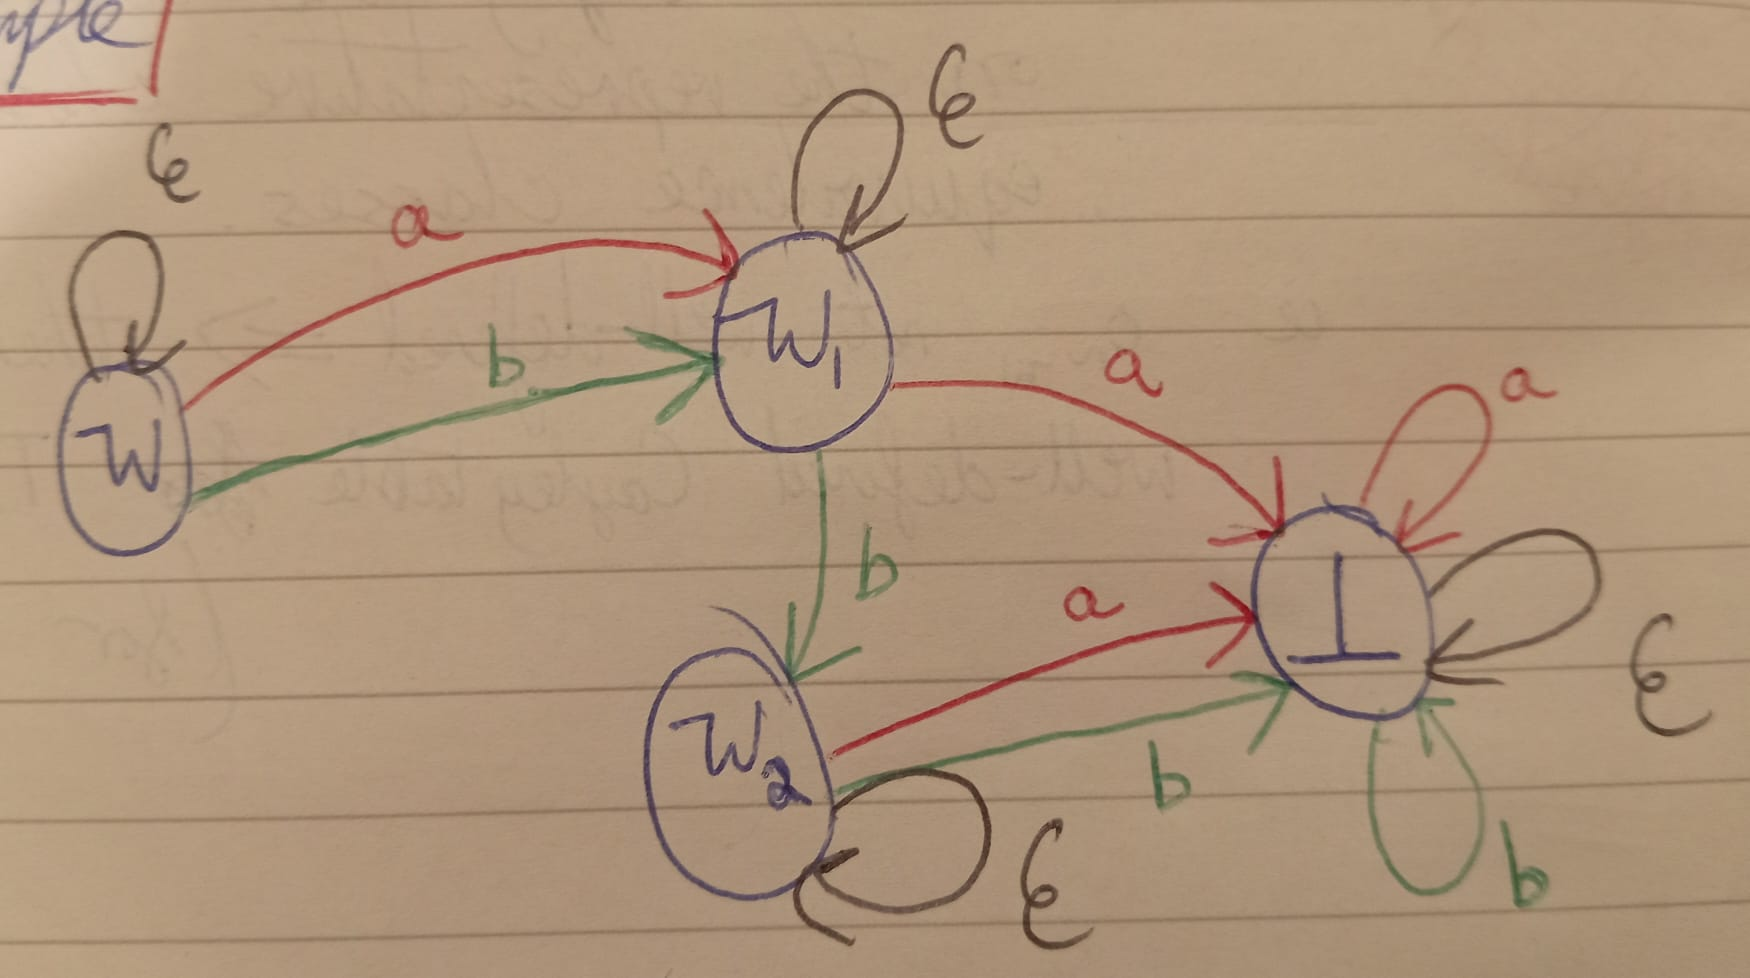
\includegraphics[width=0.5\linewidth]{5BeyondSBDRL/LocalAlgebras/Images/circ_sim_w_not_well_defined_does_not_mean_no_associativity_counter_example.jpeg}
        \caption{
        \draftnote{blue}{To do}{Improve caption.}
        }
    \end{figure}}
    \begin{table}[H]
        \centering
        \begin{tabular}{c|cccc}
            $\hat{\circ}$   & $w$       & $w_{1}$   & $w_{2}$   & $\bot$ \\
            \hline
            $\epsilon$      & $w$       & $w_{1}$   & $w_{2}$   & $\bot$ \\
            $\hat{a}$       & $w_{1}$   & $\bot$   & $\bot$   & $\bot$ \\
            $\hat{b}$       & $w_{1}$   & $w_{2}$   & $\bot$   & $\bot$
        \end{tabular}
        \caption{
        \draftnote{blue}{To do}{Improve caption.}
        }
    \end{table}

    \item \textbf{Show $\circ_{\sim_{w}}$ not well-defined.}
    From $\hat{\circ}$ we can see that
    \begin{equation}
        [a]_{\sim_{w}} = [b]_{\sim_{w}}
    \end{equation}
    Testing the well-definedness of $\circ_{\sim}$ using $[a]_{\sim_{w}} = [b]_{\sim_{w}}$ and $[a]_{\sim_{w}} = [a]_{\sim_{w}}$ gives
    \begin{align}
        & (b \circ a) \ast w = b \ast (a \ast w) = b \ast w_{1} = w_{2} \\
        & (a \circ a) \ast w = a \ast (a \ast w) = a \ast w_{1} = \bot \\
        \implies & [b \circ a]_{\sim_{w}} \neq [a \circ a]_{\sim_{w}} \\
        \implies & \circ_{\sim_{w}} \; \text{not well defined}
    \end{align}

    \item \textbf{Number of unique Cayley table constructions.}
    Using our algorithms described in \draftnote{blue}{To do}{[sections ????]}, we generate the elements of $(\hat{A}^{*}/\sim)_{w}$ and $\hat{A}^{*}/\sim_{w}$ for our example:
    \begin{align}
        & (\hat{A}^{*}/\sim)_{w} = \{ [\epsilon]_{\sim}, [a]_{\sim}, [b]_{\sim}, [aa]_{\sim}, [ba]_{\sim} \} \\
        & \hat{A}^{*}/\sim_{w} = \{ [\epsilon]_{\sim_{w}}, [a]_{\sim_{w}}, [aa]_{\sim_{w}}, [ba]_{\sim_{w}} \}
    \end{align}
    We have the following equivalence classes of $\hat{A}^{*}$ under $\sim_{w}$:
    \begin{align}
        & [\epsilon]_{\sim_{w}} = \{ \epsilon \} \quad (w \mapsto w) \\
        & [a]_{\sim_{w}} = \{ a, b \} \quad (w \mapsto w_{1}) \\
        & [ba]_{\sim_{w}} = \{ ba, bb \} \quad (w \mapsto w_{2}) \\
        & [aa]_{\sim_{w}} = \{ aa, bbb, abb \} \\
        & \cup \{ \text{any sequence suffixed with $aa$, $bbb$, or $abb$} \} \quad (w \mapsto \bot)
    \end{align}
    We've not included sequences containing $\epsilon$ composed with minimum actions explicitly in our equivalence classes since these sequences are not relevant to our analysis because $\epsilon$ always returns the world state it is applied on (i.e., $[\epsilon \circ x]_{\sim_{w}} = [x]_{\sim_{w}}$ and $[x \circ \epsilon]_{\sim_{w}} = [x]_{\sim_{w}}$ for all $x \in \hat{A}^{*}$).

    We can use \cref{prp:num_unique_cayley_table_constructions_is_product} to calculate the number $|\mathcal{C}|$ of unique Cayley table constructions of $(\hat{A}^{*}/\sim_{w}, \circ_{\sim_{w}})$:
    \begin{equation}
        |\mathcal{C}| = \prod_{j \in J} m_{j} = (1)(2)(1)(1) = 2
    \end{equation}

    \item \textbf{Find unique Cayley table constructions.}
    The local equivalence class $[a]_{\sim_{w}} \in \hat{A}^{*}/\sim_{w}$ is the only local equivalence class that contains more than one global equivalence class in $(\hat{A}^{*}/\sim)_{w}$.
    This means both unique Cayley table constructions will be generated by changing the representative element of $[a]_{\sim_{w}}$ to be representative elements of each of the global equivalence classes in $[a]_{\sim_{w}}$.

    Let $T([a]_{\sim})$ be the Cayley table construction that uses $a$ as the representative element of $[a]_{\sim_{w}}$, and let $T([b]_{\sim})$ be the Cayley table construction that uses $b$ as the representative element of $[a]_{\sim_{w}}$.
    \begin{table}[H]
        \centering
        \begin{tabular}{c|cccc}
            $\circ_{\sim_{w}}$              & $[\epsilon]_{\sim_{w}}$     & $\bm{[a]_{\sim_{w}}}$   & $[aa]_{\sim_{w}}$   & $[ba]_{\sim_{w}}$ \\
            \hline
            $[\epsilon]_{\sim_{w}}$        & $[\epsilon]_{\sim_{w}}$      & $\bm{[a]_{\sim_{w}}}$    & $[aa]_{\sim_{w}}$   & $[ba]_{\sim_{w}}$ \\
            $\bm{[a]_{\sim_{w}}}$          & $\bm{[a]_{\sim_{w}}}$        & $\bm{[aa]_{\sim_{w}}}$   & $[aa]_{\sim_{w}}$   & $[aa]_{\sim_{w}}$ \\
            $[aa]_{\sim_{w}}$              & $[aa]_{\sim_{w}}$            & $[aa]_{\sim_{w}}$   & $[aa]_{\sim_{w}}$   & $[aa]_{\sim_{w}}$ \\
            $[ba]_{\sim_{w}}$              & $[ba]_{\sim_{w}}$            & $[aa]_{\sim_{w}}$   & $[aa]_{\sim_{w}}$   & $[aa]_{\sim_{w}}$ \\
        \end{tabular}
        \caption{
        $T([a]_{\sim})$.
        \draftnote{blue}{To do}{Improve caption.}
        }
    \end{table}
    \begin{table}[H]
        \centering
        \begin{tabular}{c|cccc}
            $\circ_{\sim_{w}}$              & $[\epsilon]_{\sim_{w}}$     & $\bm{[b]_{\sim_{w}}}$   & $[aa]_{\sim_{w}}$   & $[ba]_{\sim_{w}}$ \\
            \hline
            $[\epsilon]_{\sim_{w}}$        & $[\epsilon]_{\sim_{w}}$      & $\bm{[b]_{\sim_{w}}}$    & $[aa]_{\sim_{w}}$   & $[ba]_{\sim_{w}}$ \\
            $\bm{[b]_{\sim_{w}}}$          & $\bm{[b]_{\sim_{w}}}$        & $\bm{[ba]_{\sim_{w}}}$ & $[aa]_{\sim_{w}}$ & $[aa]_{\sim_{w}}$ \\
            $[aa]_{\sim_{w}}$              & $[aa]_{\sim_{w}}$            & $[aa]_{\sim_{w}}$   & $[aa]_{\sim_{w}}$   & $[aa]_{\sim_{w}}$ \\
            $[ba]_{\sim_{w}}$              & $[ba]_{\sim_{w}}$            & $[aa]_{\sim_{w}}$   & $[aa]_{\sim_{w}}$   & $[aa]_{\sim_{w}}$ \\
        \end{tabular}
        \caption{
        $T([b]_{\sim})$.
        \draftnote{blue}{To do}{Improve caption.}
        }
    \end{table}
    
    \item \textbf{Properties of the unique Cayley table constructions.}
    \begin{table}[H]
        \centering
        \begin{tabular}{l|c}
        \textbf{Property} & \textbf{Present?} \\
        \hline
        Associative & Y \\
        Identity & Y \\
        Inverses & N \\
        \hline
        Commutative & Y \\
        \end{tabular}
        \caption{
        Properties of $T([a]_{\sim})$.
        \draftnote{blue}{To do}{Sort table formatting.}
        }
    \end{table}
    
    \begin{table}[H]
        \centering
        \begin{tabular}{l|c}
        \textbf{Property} & \textbf{Present?} \\
        \hline
        Associative & Y \\
        Identity & Y \\
        Inverses & N \\
        \hline
        Commutative & Y \\
        \end{tabular}
        \caption{
        Properties of $T([b]_{\sim})$.
        \draftnote{blue}{To do}{Sort table formatting.}
        \draftnote{blue}{To do}{Check this algorithmically.}
        }
    \end{table}

    \item \textbf{Conclusion.}
    Since $T([a]_{\sim})$ and $T([b]_{\sim})$ both satisfy the associativity property, every unique Cayley table construction of $(\hat{A}^{*}/\sim_{w}, \circ_{\sim_{w}})$ for our example world satisfies the associativity property.
\end{enumerate}
\end{proof}


\draftnote{blue}{To do}{
Code to calculate the number of unique Cayley table constructions and then to generate them.
\textbf{To calculate:}
\begin{enumerate}
    \item Generate $\hat{A}^{*}/\sim_{w}$ and $(\hat{A}^{*}/\sim)_{w}$.
    \item Work out which local equivalence class of $\hat{A}^{*}/\sim_{w}$ that each element of $(\hat{A}^{*}/\sim)_{w}$ is in.
    \item Find product.
\end{enumerate}
\textbf{To generate:}
\begin{enumerate}
    \item Generate $\hat{A}^{*}/\sim_{w}$ and $(\hat{A}^{*}/\sim)_{w}$.
    \item Work out which local equivalence class of $\hat{A}^{*}/\sim_{w}$ that each element of $(\hat{A}^{*}/\sim)_{w}$ is in.
    \item Generate all distinct global-class choices.
    \item Generate Cayley table constructions.
\end{enumerate}
}

\begin{proposition}
    A Cayley table construction of $(\hat{A}^{*}/\sim_{w}, \circ_{\sim_{w}})$ satisfies the associativity property $\nRightarrow$ $\circ_{\sim_{w}}$ is well-defined.
\end{proposition}
\begin{proof}
    Proof by example using the same example as given in \cref{prp:circ_sim_w_not_well_defined_does_not_mean_no_associativity}, which is a world where $\circ_{\sim_{w}}$ is not well-defined and the associativity property is satisfied by a Cayley table construction of $(\hat{A}^{*}/\sim_{w}, \circ_{\sim_{w}})$.
\end{proof}


\begin{proposition}
    (1) The Cayley table constructions of $(\hat{A}^{*}/\sim_{w}, \circ_{\sim_{w}})$ do not always satisfy the identity property, but (2) there is always at least one Cayley table construction of $(\hat{A}^{*}/\sim_{w}, \circ_{\sim_{w}})$ that satisfies the identity property, which is when $\epsilon$ is used as the representative of $[\epsilon]_{\sim_{w}}$.
\end{proposition}
\begin{proof}
    (1) by example, (2) by proof.
    \begin{enumerate}[(1)]
        \item \textbf{Proof by example.}
        \begin{enumerate}
            \item \textbf{Set up.}
                \draftnote{blue}{To do}{Give this world a Greek letter.}
                Consider a world-agent pair $\mathscr{W}-\mathscr{A}$ with $W = \{ w, w', w'', \bot \}$, $\hat{A} = \{a, b\}$, and $\hat{\circ}$ given by
                \begin{table}[H]
                    \centering
                    \begin{tabular}{c|cccc}
                        $\hat{\circ}$   & $w$       & $w'$      & $w''$     & $\bot$ \\
                        \hline
                        $\epsilon$      & $w$       & $w'$      & $w''$     & $\bot$ \\
                        $a$             & $w'$      & $\bot$    & $\bot$    & $\bot$ \\
                        $b$             & $w$       & $w''$     & $\bot$    & $\bot$
                    \end{tabular}
                    \caption{
                    \draftnote{blue}{To do}{Improve caption.}
                    }
                \end{table}
            \item \textbf{Construct Cayley table with no identity.}
            We will now construct a Cayley table for $(\hat{A}^{*}/\sim_{w}, \circ_{\sim_{w}})$ that does not satisfy the identity property.
            We choose to use $b \in \hat{A}^{*}$ as the representative element for $[\epsilon]_{\sim_{w}}$.
            \begin{table}[H]
                \centering
                \begin{tabular}{c|cccc}
                    $\circ_{\sim_{w}}$  & $[b]_{\sim_{w}}$  & $[a]_{\sim_{w}}$   & $[ba]_{\sim_{w}}$  & $[aa]_{\sim_{w}}$ \\
                    \hline
                    $[b]_{\sim_{w}}$    & $[b]_{\sim_{w}}$  & $[ba]_{\sim_{w}}$  & $[aa]_{\sim_{w}}$  & $[aa]_{\sim_{w}}$ \\
                    $[a]_{\sim_{w}}$    & $[a]_{\sim_{w}}$  & $[aa]_{\sim_{w}}$  & $[aa]_{\sim_{w}}$  & $[aa]_{\sim_{w}}$ \\
                    $[ba]_{\sim_{w}}$   & $[ba]_{\sim_{w}}$ & $[aa]_{\sim_{w}}$  & $[aa]_{\sim_{w}}$  & $[aa]_{\sim_{w}}$ \\
                    $[aa]_{\sim_{w}}$   & $[aa]_{\sim_{w}}$ & $[aa]_{\sim_{w}}$  & $[aa]_{\sim_{w}}$  & $[aa]_{\sim_{w}}$
                \end{tabular}
                \caption{
                \draftnote{blue}{To do}{Improve caption.}
                }
            \end{table}
            From inspecting the Cayley table construction we can see it does not satisfy the identity property.\footnote{
            In fact, any world where there is some action $a \in \hat{A}^{*}$ that satisfies
            \begin{equation}
                [a]_{\sim_{w}} = [\epsilon]_{\sim} \quad \text{but} \; [a]_{\sim} \neq [\epsilon]_{\sim}
            \end{equation}
            will have at least one Cayley table construction that does not satisfy the identity property.
            \draftnote{blue}{Consider}{Prove this explicitly?}
            }
        \end{enumerate}

        \item \draftnote{red}{UP NEXT}{}
    \end{enumerate}
\end{proof}



\draftnote{blue}{To do}{
Show example using $\mathscr{W}_{\beta}$ with identity treatment of when switching the representative element leads to a different Cayley table construction.
}
\draftnote{blue}{To do}{
$\circ_{\sim_{w}}$ is well-defined on $\hat{A}^{*}/\sim_{w}$ $\implies$ $[\epsilon]$ is identity element of $\circ_{\sim_{w}}$ on $\hat{A}^{*}/\sim_{w}$.
}
\draftnote{blue}{Consider}{
Do elements of the identity class form a group in some way ?
}

%%%%%%%%%%%%%%%%%%%%%%%%%%%%%%%%%%%%%%%
\subsection{
What have we discovered ?
}
\draftnote{green}{To do}{
\begin{enumerate}
    \item Table summarising the associativity vs well-defined properties.
    \item Associativity breaking as an indicator that $\circ_{\sim_{w}}$ is not well-defined.
    \item We cannot guarantee that any of the group properties are satisfied or are not satisfied in a Cayley table construction of $(\hat{A}^{*}/\sim_{w}, \circ_{\sim_{w}})$. - these are pseudo algebras ?
\end{enumerate}
}


%%%%%%%%%%%%%%%%%%%%%%%%%%%%%%%%%%%%%%%
\subsection{
Homogenous vs inhomogeneous actions
}
\draftnote{green}{To do}{
\begin{enumerate}
    \item Define homogeneous actions (+ inhomogeneous actions).
    \item Define action-homogeneous worlds (+ action-inhomogeneous worlds)
    \begin{itemize}
        \item Do we want action-homogeneous worlds to be a subset of action-inhomogeneous worlds?
    \end{itemize}
    \item \textbf{Proof:} $\circ_{\sim_{w}}$ is well-defined in action-homogeneous worlds.
    \begin{itemize}
        \item Is $\circ_{\sim_{w}}$ well defined for composition of homogeneous actions even in action inhomogeneous worlds ?
    \end{itemize}
    \item \textbf{Homogenous actions proofs}
    \begin{enumerate}
        \item \textbf{Corollary from definition.}
        $[\epsilon]$ is a homogeneous action.
        \item \textbf{Corollary from definition.}
        Either a homogeneous action is always defined or always undefined.
        \item \textbf{Corollary from definition.}
        Either two actions are identity or not.
        \item \textbf{Proof.}
        Global consistent inverse means both actions are homogeneous ?
        \item \textbf{Proof.}
        For two homogeneous actions $a, a' \in \hat{A}^{*}$, $a \sim_{w} a'$ $\implies$ $a \sim a'$.
        \begin{itemize}
            \item NB: this makes the algebra much easier to learn.
        \end{itemize}
    \end{enumerate}
    \item \textbf{Action-homogeneous worlds proofs}
    \begin{enumerate}
        \item \textbf{Proof.}
        Action-homogeneous world $\iff$ $(\hat{A}^{*}/\sim_{w_{i}}, \circ_{\sim_{w_{i}}})$'s are isomorphic to each other.
        \item \textbf{Proof.}
        Action-homogeneous world $\iff$ $(\hat{A}^{*}/\sim_{w_{i}}, \circ_{\sim_{w_{i}}})$ are isomorphic to $(\hat{A}^{*}/\sim, \circ_{\sim})$.
        \begin{itemize}
            \item \textbf{Corollary.}
            $|(\hat{A}^{*}/\sim, \circ_{\sim})| = |W^{\bot}|$.
        \end{itemize}
        \item \textbf{Proof.}
        World is action-homogeneous and reversible $\implies$ $(\hat{A}^{*}/\sim, \circ_{\sim})$ (and therefore local algebra) is a group.
        \item \textbf{Proof.}
        World is action-homogeneous and reversible \textbf{does not} $\impliedby$ $(\hat{A}^{*}/\sim, \circ_{\sim})$ (and therefore local algebra) is a group.
        (i.e., Is it possible to get a world with a global group algebra $\sim$ but that's not action homogeneous ?)
        \begin{itemize}
            \item I think yes - find counter example.
        \end{itemize}
    \end{enumerate}
\end{enumerate}
}


What property of the world $\mathscr{W}_{\alpha}$ means that $(\hat{A}^{*}/\sim_{w_{i}}, \circ_{\sim_{w_{i}}})$ is isomorphic to $(\hat{A}^{*}/\sim, \circ_{\sim})$?



\draftnote{blue}{old}{
World condition ref[wldcon:action-homogeneity] means that action sequences have the same result for any initial world state.
Essentially, this means that the world looks the same from any world state with respect to the relationships of actions.
We call worlds with world condition ref[wldcon:action-homogeneity] \textit{action-homogeneous worlds}.
}





\draftnote{blue}{Old action homogeneity definition}{
For every pair $(w_{1}, w_{2}) \in W^{2}$, there exists a bijective map $\sigma_{(w_{1},w_{2})}: W \to W$ such that $\sigma_{(w_{1},w_{2})}(w_{1})=w_{2}$ and such that:
\begin{enumerate}
    \item for every $d \in D_{A}$ with $d: s(d) \xrightarrow{a} t(d)$, there exists a $d' \in D_{A}$ with $d': \sigma_{(w_{1}, w_{2})}(s(d)) \xrightarrow{a} \sigma_{(w_{1}, w_{2})}(t(d))$;
    % Is this part needed --> implied by first condition due to $\sigma$ being a bijection ?
    \item for every $d \in D_{A}$ with $d: s(d) \xrightarrow{a} t(d)$, there exists a $d' \in D_{A}$ with $d': \sigma^{-1}_{(w_{1}, w_{2})}(s(d)) \xrightarrow{a} \sigma^{-1}_{(w_{1}, w_{2})}(t(d))$.
\end{enumerate}
}

\draftnote{blue}{Consider}{
\textbf{Generalisation and action-homogeneous worlds.}
If we know that, from a particular initial state, a particular sequence of actions has a particular outcome and we know that a different sequence of actions from the same initial state has the same outcome then we know that those two action sequences will have the same outcome in from every initial state (and therefore will be equivalent?!).
Illustrate this using the counter-example - see PhD Notebook 1 notes.
}
\draftnote{blue}{Consider}{
Subsection on homogenous irreversible actions?
Colours changing infinitely ?
Not possible in practice with non ideal sensors - there are parts around each observation state that the sensors cannot distinguish.
You get spheres of indistinguishability around each observation state; distinguishable states appear at the intersection of these spheres???
}
\draftnote{blue}{Consider}{
Hypothesis: action-homogeneous worlds are easier to learn.
Can we design a method that an agent could use to work out the algebra for these worlds ?
Could use the (old) algorithm we developed because each time we move to a new state it's as if we're returning to where we began (kinda - states are still distinct).
}

%%%%%%%%%%%%%%%%%%%%%%%%%%%%%%%%%%%%%%%
\subsection{
An easy mistake: \autocite{caselles2020sensory}
}
\draftnote{green}{To do}{
\begin{enumerate}
    \item Explain mistake in \autocite{caselles2020sensory}.
    \begin{itemize}
        \item Mistake due to confusion between globally reversible vs consistently globally reversible vs having a consistent global inverse (which is the group property) --> reference proof that global reversibility implies consistent global inverse for certain worlds.
        \item Made more difficult to spot because the world without objects in is action homogeneous and so (assuming finite) globally reversible $\implies$ having a consistent global inverse (see done proposition earlier) + because our world appears locally action homogeneous.
    \end{itemize}
    \item Check the PhD thesis that \autocite{caselles2020sensory} cited.
\end{enumerate}
}



